\section{Result: Standard Network}  \label{s:N_II:std_net}

\vspace{3mm}
% \noindent\rule{17cm}{0.2pt}
\fbox {
    \parbox{\linewidth}{
      \begin{itemize}
        \item Network communities traced to splitting the ABS-Ca and P0 datasets 
        \item ModCon selected genes are significantly expressed in the new healthy splits
        \item First attempt to stratify the MIBC using the healthy network
      \end{itemize}
    }
}
\vspace{3mm}

% Non-tum split
\subsection{Healthy splits} \label{s:N_II:std}

% Introduction to the work
The healthy dataset consists of three different tissue types: undifferentiated (UD), \acrshort{absCa} differentiated (\acrshort{absCa}) and freshly isolated cells (P0); see \cref{s:lit:datasets_used} for an introduction to the datasets. The new network pipeline, \cref{s:N_II:methods}, was applied to the non-tumour dataset to test if the approach can stratify the data into the three tissue differentiated status.

% Introduce the methods used to get the groups
To achieve this, the same filtering as in \cref{s:cs:pre-processing} was used to select the 5000 most varied genes, then the network pipeline is applied. The MEVs were then analysed with both the cluster analysis described in \cref{s:cs:methods} and the Morpheus software \citep{Broad-Institute2016-tn}. Due the small number of samples (88) the latter was preferred to visualise and perform the hierarchical clustering, with average linkage and cosine distance. Applying quantile normalisation on the dataset aid the visualisation of the heatmap and resulted in \cref{fig:N_II:morph_non_tum}. There are four metadata shown at the top of the figure: 
\begin{itemize}
    \item Biological sex: Male (M), F (Female)
    \item \acrfull{nhu}: ABS-Calcium, undifferentiated and freshly isolated
    \item Subset name: Bladder differentiated (B-Diff), (NR-DIF), Urothelium differentiated (Uro-D), P0 (Uro-P0) and undifferentiated (Uro-UD)
    \item Diagnosis - \acrfull{ic}, \acrfull{cc}, \acrfull{nsUI},  \acrfull{nvh}, \acrfull{oab}, Prolapse, \acrfull{ruti}, \acrfull{sui}
\end{itemize} 

% Heatmap -
From the heatmap in \cref{fig:N_II:morph_non_tum} it can be seen that the hierarchical clustering finds the three distinct groups of tissue differentiation, which further validates the network approach. On top of that, as the dendrogram cut is increased to 7, there are other subgroups: a male subtype by cluster 5 and two main subtypes of the differentiated samples (6 and 7); clearer displayed in \cref{fig:N_II:non_tum_sankey_comp}. The P0 subgroups are also split into two if the dendrogram cut is further increased, while there are 3 P0 samples which are clustered differently from the rest of the P0 samples. 

\begin{figure}[!t]    
    \centering
    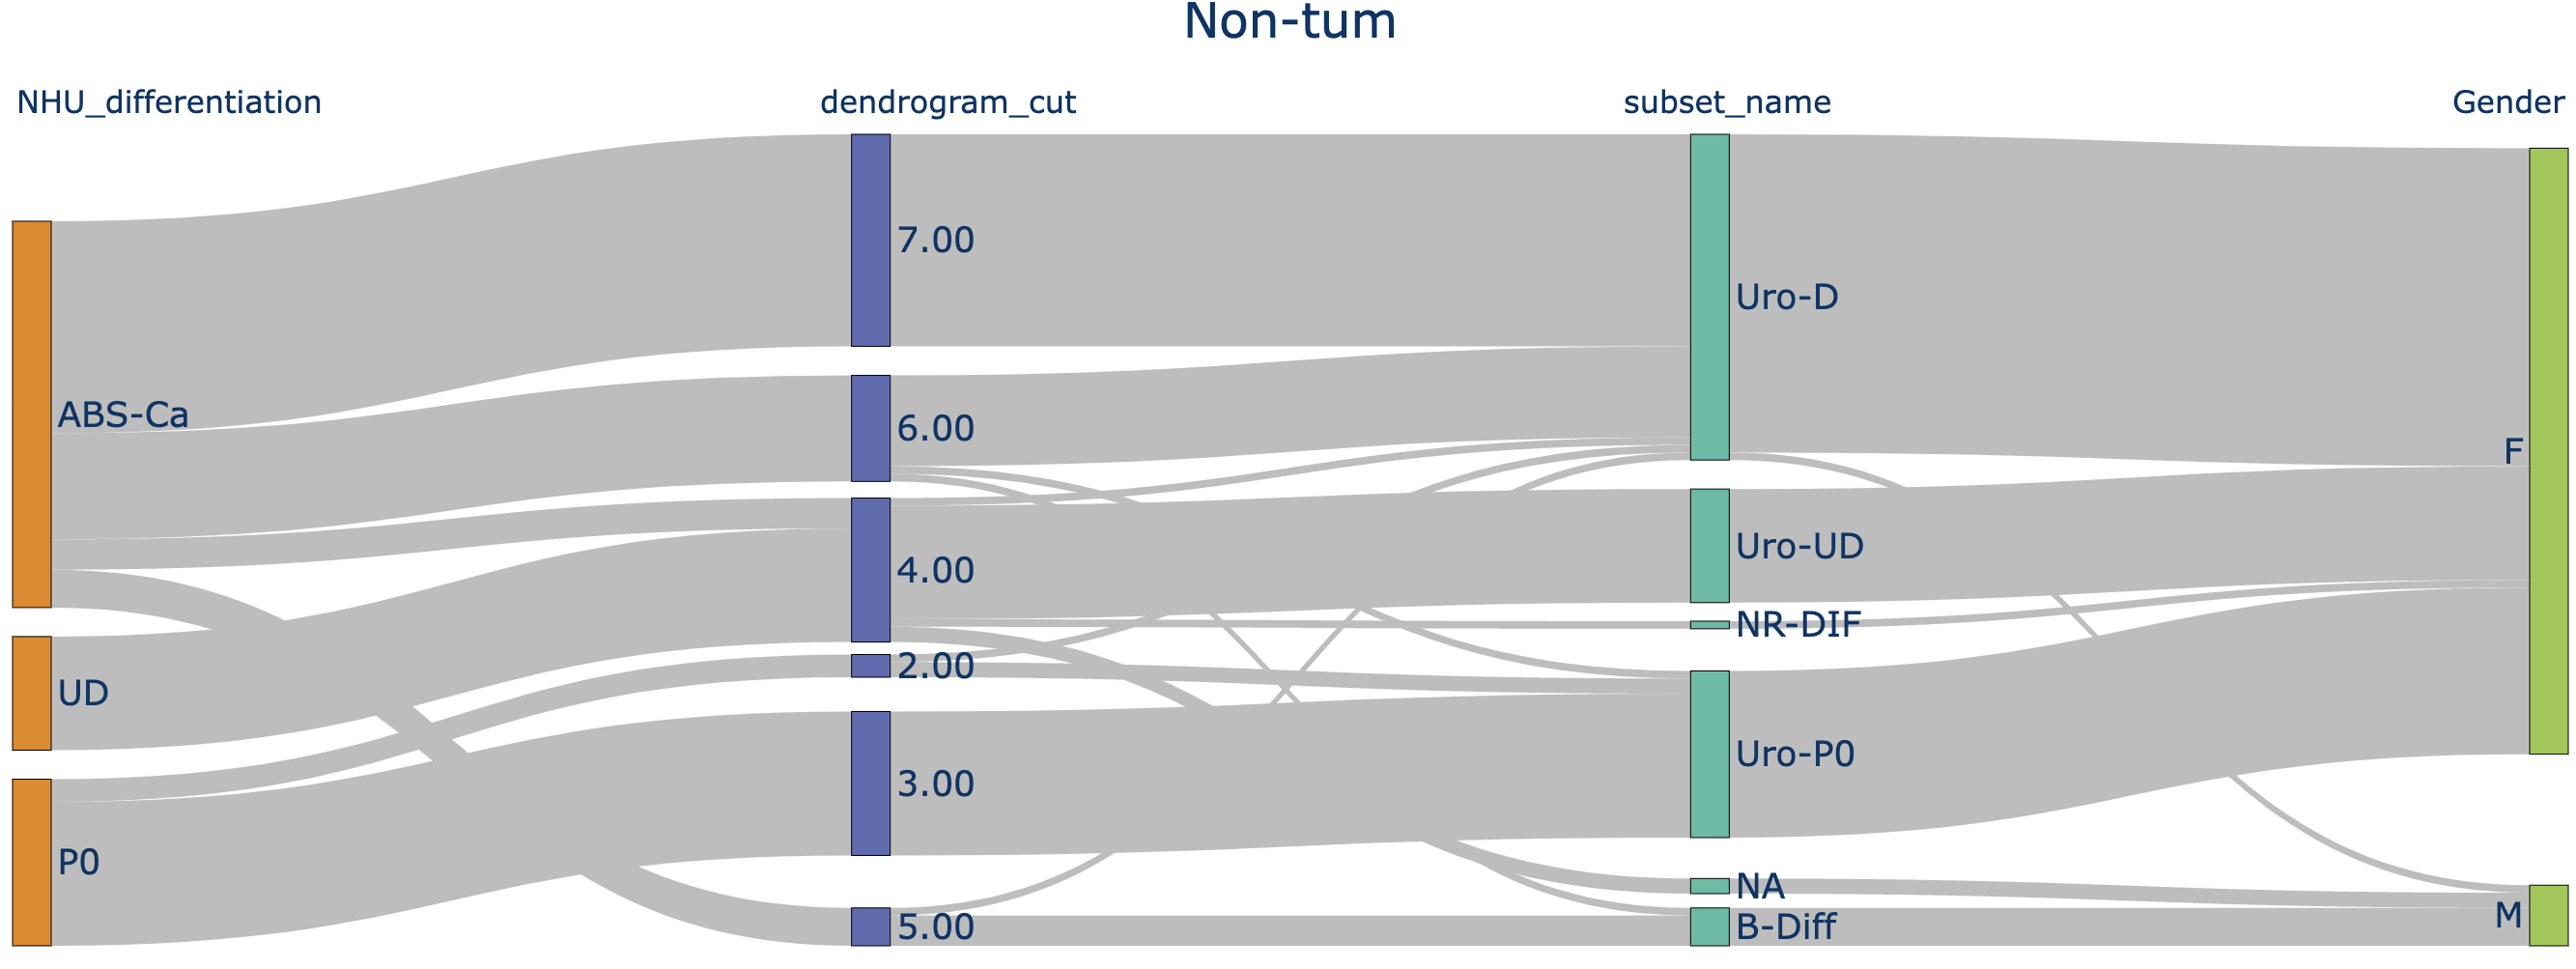
\includegraphics[width=1.0\textwidth,keepaspectratio]{Sections/Network_II/resources/non_tum/non_tum_split.png}
    \caption[Split of the non-tumour dataset]{Sankey plot that shows the non-tumour dataset split compared with the metadata for NHU differentiated status, subset and biological sex. It shows that the new network pipeline can find the three distinct differentiated tissues with further divisions.}
    \label{fig:N_II:non_tum_sankey_comp}
\end{figure}

% Explain the P0
The three 'isolated' P0 samples: Y2306, Y2439 and Y2383 have a high immune response which was highlighted by independent clinical histopathologist review at St James's University Hospital, Leeds. The male predominant group (5): Y815A-Bl, Y836B-Bl, Y499B-Bl, Y929B-Bl are paediatric samples which may explain why were grouped separately. However, Y719B-Bl is also a male paediatric sample but was grouped with the large differentiated subtype (7); is the only male sample on the right hand side of the heatmap. \acrfull{dea} and \acrfull{gsea} were used to further analyse the subgroups but there were not significant differences, including chromosome Y specific signatures.

% Talk about the male differentiated samples that are pedriatic
The ABS-Ca samples are split into a smaller (14 samples) and a large (28 samples) group; \cref{fig:N_II:non_tum_sankey_comp}. From inspecting the heatmap, \cref{fig:N_II:morph_non_tum}, the smaller differentiated group is enriched in communities 19, 1 and 29 while the large group is not. Group 7 (large group) is also enriched in communities 25 and 22,  but 6 (smaller group) has a low expression of these communities. This means, that enrichment in communities 19, 1, 29, 25 and 22 establish the differences between the two differentiated groups. This is further explored in \cref{s:N_II:diff_split}.


\begin{sidewaysfigure}
    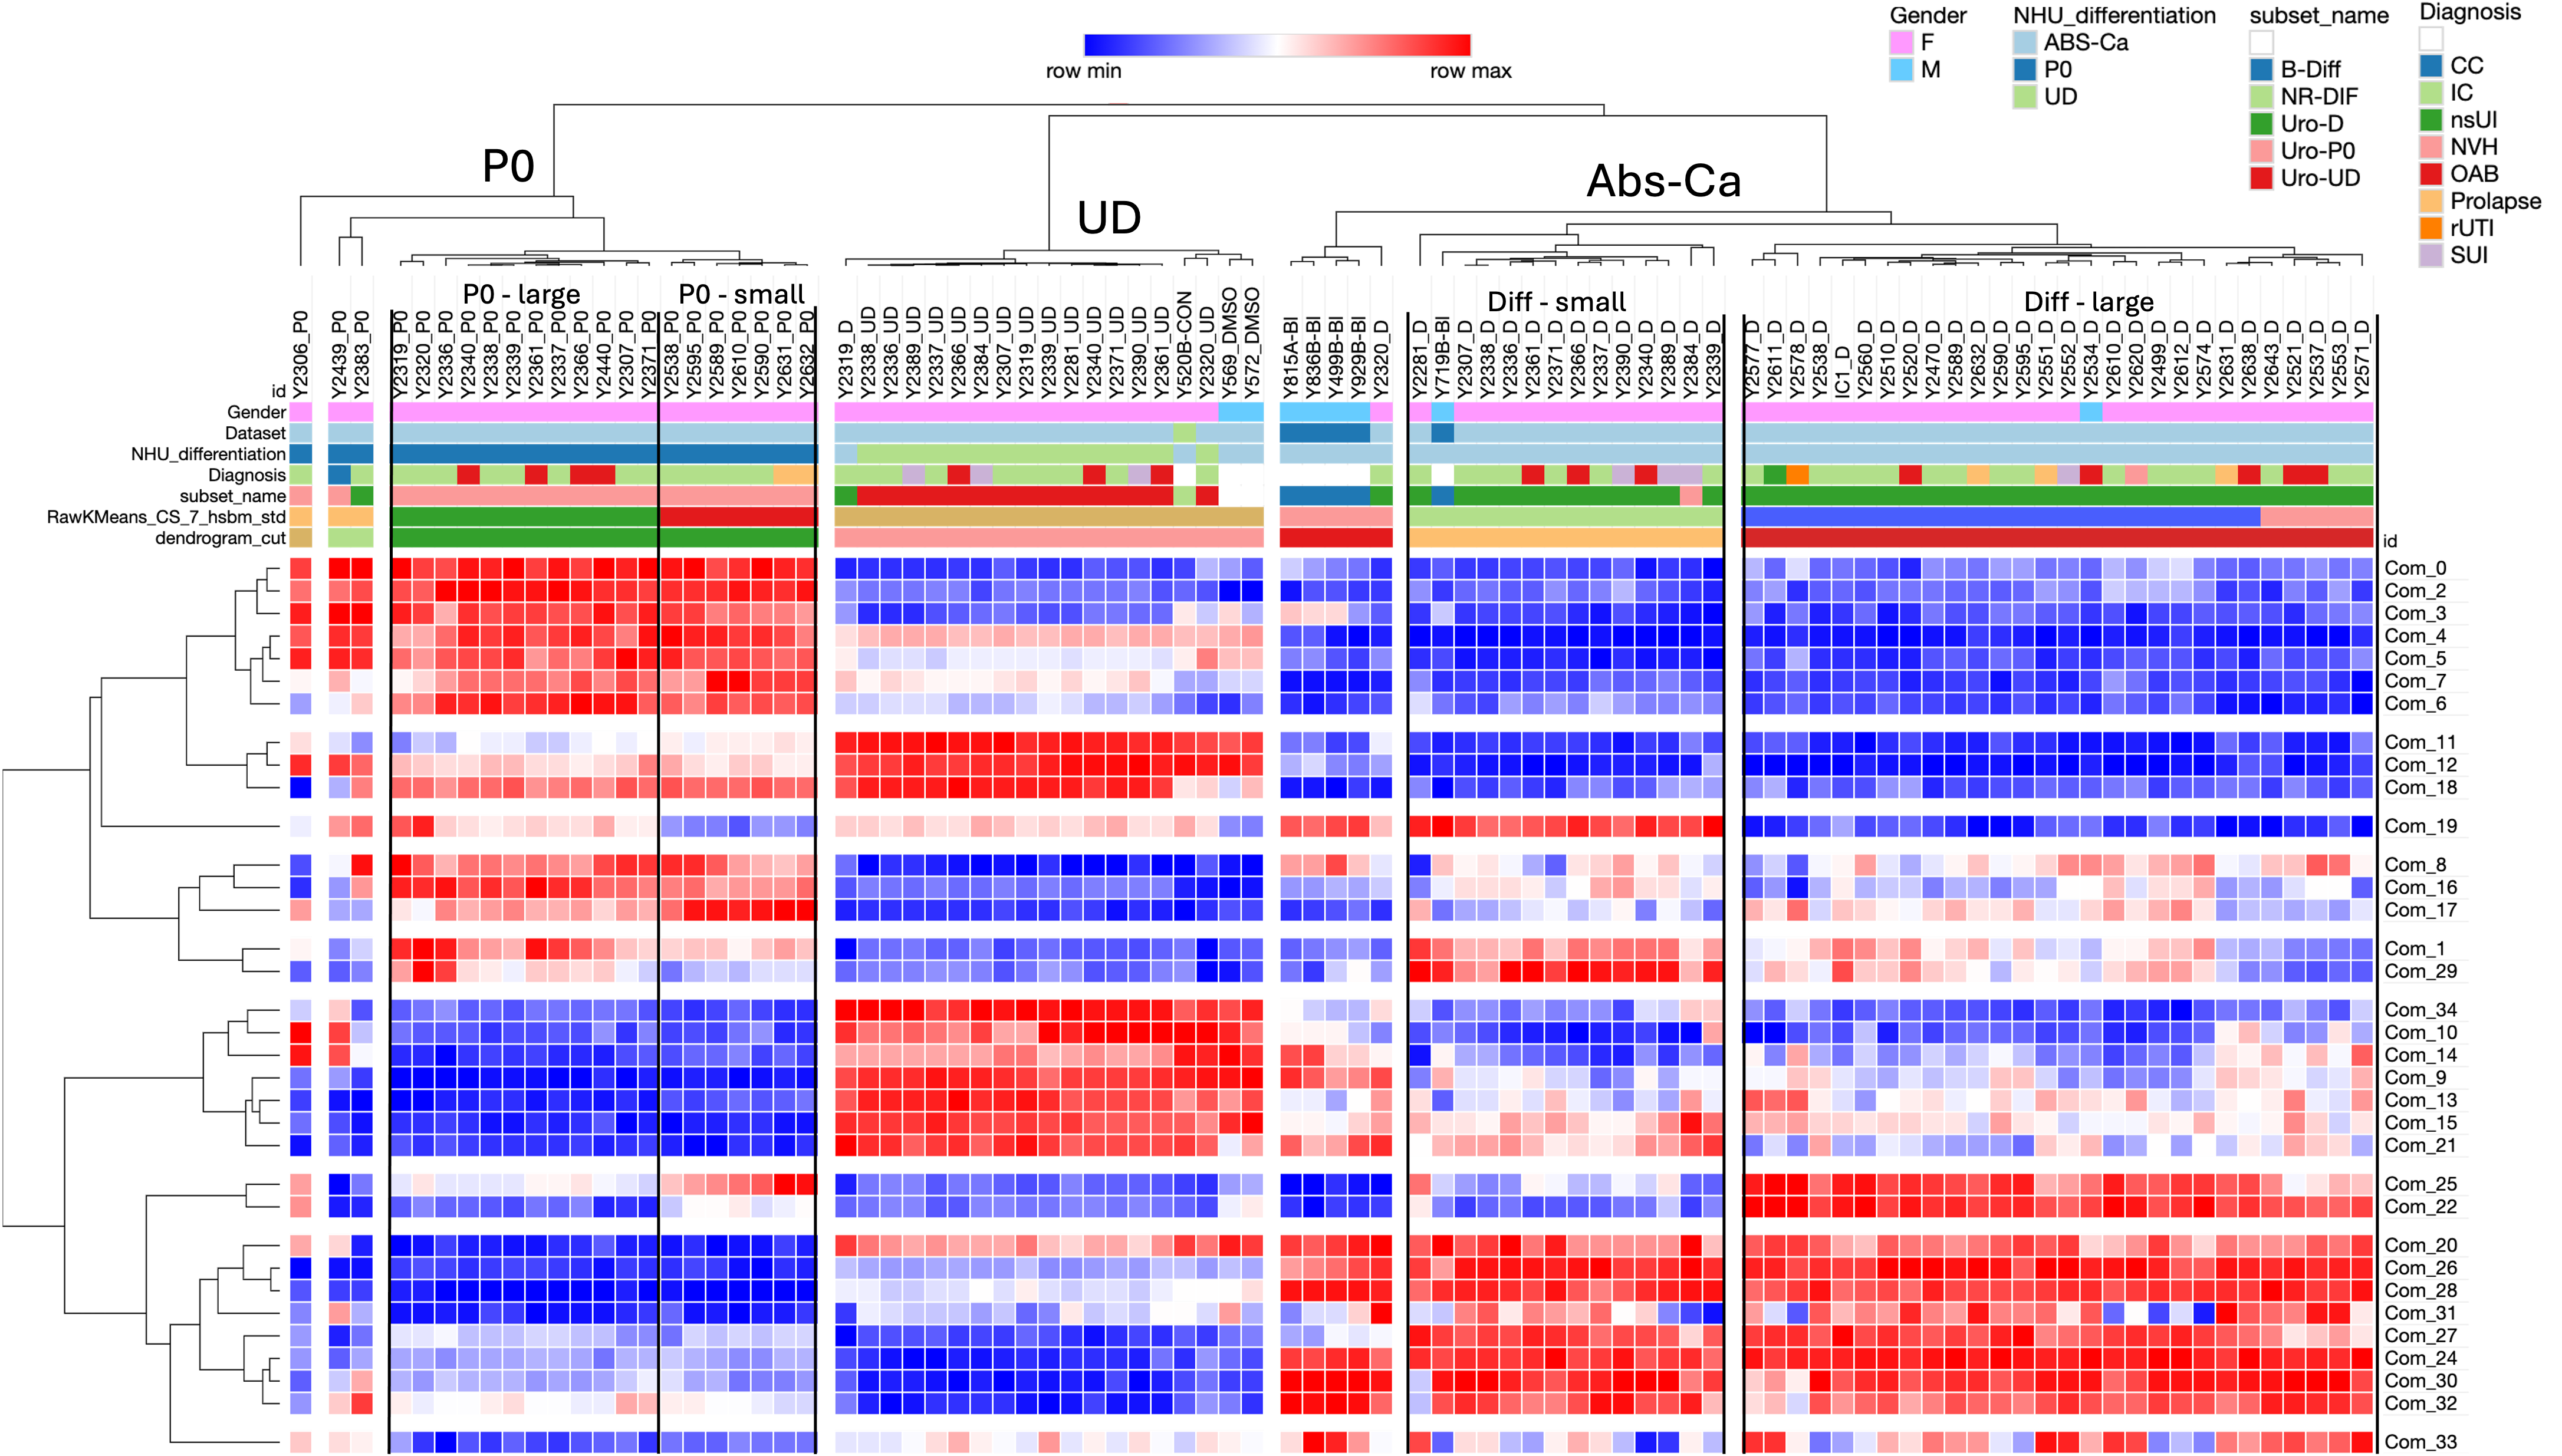
\includegraphics[width=1.0\textwidth,height=1.0\textheight,keepaspectratio]{Sections/Network_II/resources/non_tum/norm_healthy_std_3.1.png}
    \caption[Heatmap of the new non-tumour subgroups]{Heatmap showing both the groups in the non-tumour dataset and the clustered communities. Hierarchical clustering with average linkage and cosine distance is applied on the MEVs resulted from the network pipeline. There are four metadata shown at the top: Gender, NHU differentiation, subset name and the Diagnosis. }
    \label{fig:N_II:morph_non_tum}
\end{sidewaysfigure}


% P0 difference
The difference in P0 is not as evident as in the ABS-Ca samples split, but it can be seen that the smaller P0 group is enriched in 25 while the larger P0 is less so. In addition, the genes from community 19, 29 are more expressed in the larger P0 group compared to the smaller subtype. This indicate that communities 25, 19 and 29 play a role in making the difference; the differences in P0 is explored in \cref{s:N_II:p0_split}. The communities responsible to split the samples are summarised below:
\begin{itemize}
    \item \acrshort{absCa} split: 1, 19, 22, 25, 29
    \item P0 split: 19, 22, 25, 29
\end{itemize}

% ABS-Ca splits
\subsection{ABS-Ca splits} \label{s:N_II:diff_split}

% Introduce the Splits
Both the heatmap (\cref{fig:N_II:morph_non_tum}) and Sankey plot (\cref{fig:N_II:non_tum_sankey_comp}) show that the ABS-Ca differentiated samples are split into three different subtypes: 5, 6, and 7. It was mentioned earlier that group 5 consists of paediatric samples, which could explain the separation. To further explore the differences between groups 6 (small ABS-Ca) and 7 (large ABS-Ca), \acrlong{dea} was performed between the samples of the two group, method covered in \cref{s:lit:dea}. The output of DEA can be seen in \cref{fig:N_II:diff_split}, where 'Dataset' the coloured traces for 19, 1, 29, 25, and 22 represents the genes selected by ModCon for each corresponding community.

% Describe the DEA
% The ouput of the \acrshort{dea} can be seen in \cref{fig:N_II:diff_split}, where the X-axis represents the difference in gene expression ($log_2(\text{fold\_change})$), while the Y-axis shows the significance of the change given by $-log_{10}(q)$. As the name suggests, "Point(s) of interest" are the genes that are outside of the $log_2(\text{fold\_change})$ bounds (\textbf{$+/-1$}) and have a high expression difference, making them worth considering for future analysis. 

% Analysis of the volcano plot
In \cref{fig:N_II:diff_split}, the left-hand side represents the genes that are highly expressed in the larger ABS-Ca group, while the right-hand side shows the genes specific to the small ABS-Ca group. From left to right, it can be noticed that the genes selected by communities 25 (green) and 22 (purple) are specific to the larger ABS-Ca group, which is highlighted by the heatmap in \cref{fig:N_II:morph_non_tum}. However, some of the genes in community 25 do not have a much higher expression in the large ABS-Ca group, as they are closer to the middle. On the other side, genes specific to community 19 are specific to the smaller ABS-Ca group. Genes from communities 29 and 1 are more expressed in the small ABS-Ca group but are at the threshold level of not having a high expression difference.

% Concluding analysis
The analysis suggests that the up-regulation of genes from community 19 is specific to the smaller ABS-Ca group, while the genes from community 25 are specific to the larger ABS-Ca group. Communities 29 and 1 have a 'tendency' towards the smaller group, while community 22 tends towards the larger group.

% Linking to the network and communities
It is remarkable that the network pipeline, through the ModCon score, is able to select most of the genes that are significantly different between the two groups. It is worth considering that the DEA uses all the expressed genes, while the network approach considers only 5000 genes. This demonstrates that the pipeline is capable of finding significantly different genes, which can also be linked to network communities.

% Talk about ENSG
Another important observation from the selected points in the volcano plot in \cref{fig:N_II:diff_split} is that many of the highlighted genes are identified by Ensembl IDs rather than Human Genome Organisation (HUGO) names, following the pattern 'ENSG...'. This suggests that these genes are not well-characterised and could potentially reveal new biological insights. However, this also poses a challenge for further study, as these genes are more difficult to investigate.


\begin{sidewaysfigure}   
    \centering
    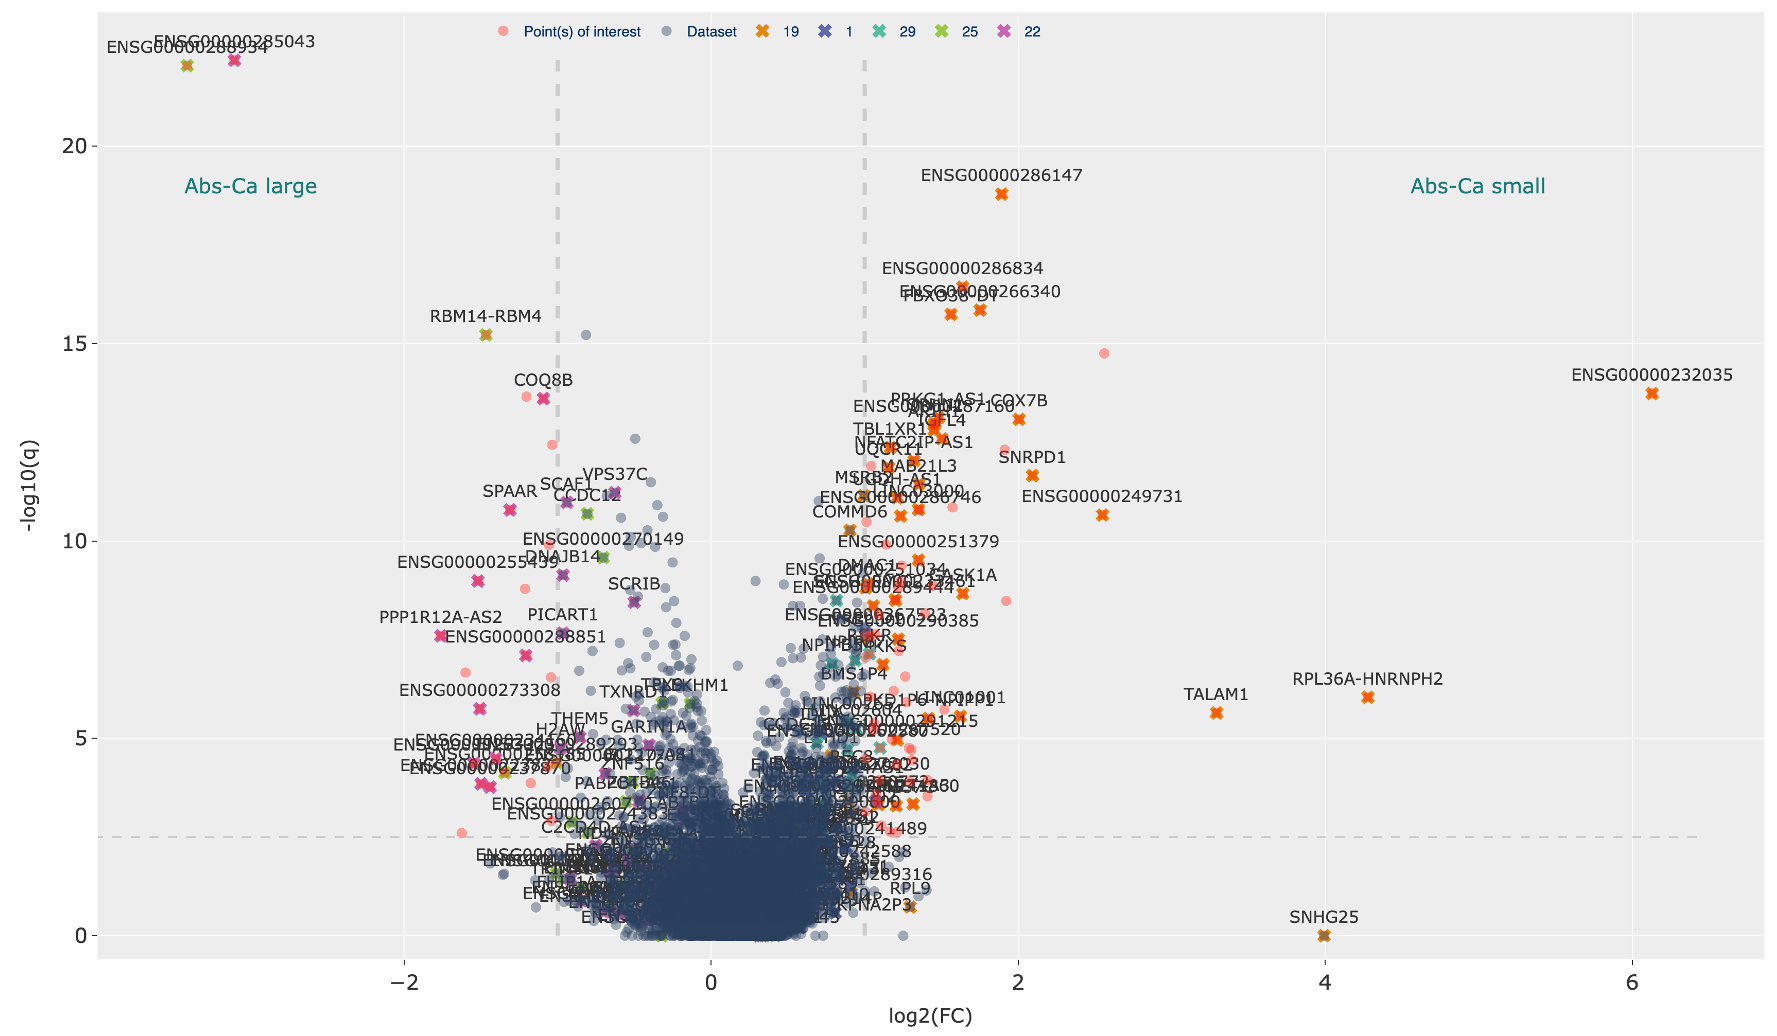
\includegraphics[width=1.0\textwidth,height=1.0\textheight,keepaspectratio]{Sections/Network_II/resources/non_tum/diff_split_dea.png}
    \caption[Volcano plot between the ABS-Ca splits]{Volcano plot showing the \acrlong{dea} for the comparison between groups 6 (small ABS-Ca) and 7 (large ABS-Ca). The X-axis represents the difference in gene expression, $log_2(\text{fold\_change})$, while the Y-axis shows the significance of the change given by $-log_{10}(q)$. The 19, 1, 29, 25, and 22 coloured points represent the genes selected by ModCon for each corresponding community. The genes on the right-hand side of the plot are those significantly expressed in the larger ABS-Ca group, while the points on the left-hand side are specific to the smaller ABS-Ca group. The volcano plot shows that the significantly expressed genes between the two ABS-Ca groups mostly consists for Ensembl IDs genes which are poorly described in the literature thus showing the potential of new biological findings.}
    \label{fig:N_II:diff_split}
\end{sidewaysfigure}


% P0 split
\subsection{P0 split} \label{s:N_II:p0_split}

% Why doing the P0
There is another split of a major differentiated tissue type, P0,  which is not as clear as the ABS-Ca groups, but present and it can be observed that communities 19, 22, 25 and 29 are driven the separation; see \cref{fig:N_II:morph_non_tum}. To study more the division in the P0 samples, the same approach was taken as in the precedent sub-section, where \acrshort{dea} is applied and the genes selected through ModCon are highlighted in the plot.

% Introducing the volcano plot
\Cref{fig:N_II:p0_split} represents the volcano plot of the DEA between the two P0 subgroups, labelled as P0 large and P0 small. The genes on the left-hand side of the plot are higher expressed in the larger group and higher these are on the Y-axis the more significant differentially expressed are. Conversely, on the right hand side are the genes representative for the smaller P0 group.

% Talk about the communities
The volcano plot confirms that the genes from communities 19 (blue) and 29 (green) are up-regulated in the larger P0 but not expressed in the other group. Conversely, the expression of genes from 25 (orange) and 22 (red) are more present in the smaller P0 compared to the larger subtype. It can also be noticed that most of the genes highlighted have predominantly Ensembl IDs denoting the novelty of the findings but also the challenge of determining their function. 

This analysis reinforce the fact that the network pipeline is capable of finding communities which drive separation in well-known groups. It also shows that ModCon extracts genes that are significantly expressed in the group division. The freshly isolated P0 samples are the only ones from the non-tumour dataset that might have an immune cell infiltration but neither of the two P0 splits exhibit immune response. 

Many of the genes found are Ensembl IDs that are poorly described in the literature and usually represent \acrfull{lncRNA}. While this type of gene does not code for proteins, there is mounting evidence that lncRNA plays a role in gene regulatory function and chromatin remodelling, both of which are relevant in the context of bladder cancer \citep{Statello2021-md}. It was also noticed in the MIBC groups found from applying cluster analysis that there are \acrlong{lncRNA} genes (\textit{DANCR, SLC16A1}) have a functional role in bladder cancer; see \cref{s:cs:basal_interp}. This suggests that the network approach can filter lncRNA, potentially adding layer of information to bladder cancer research. Tracing the genes from a subset of communities to the volcano plot is also possible.

\begin{sidewaysfigure}    
    \centering
    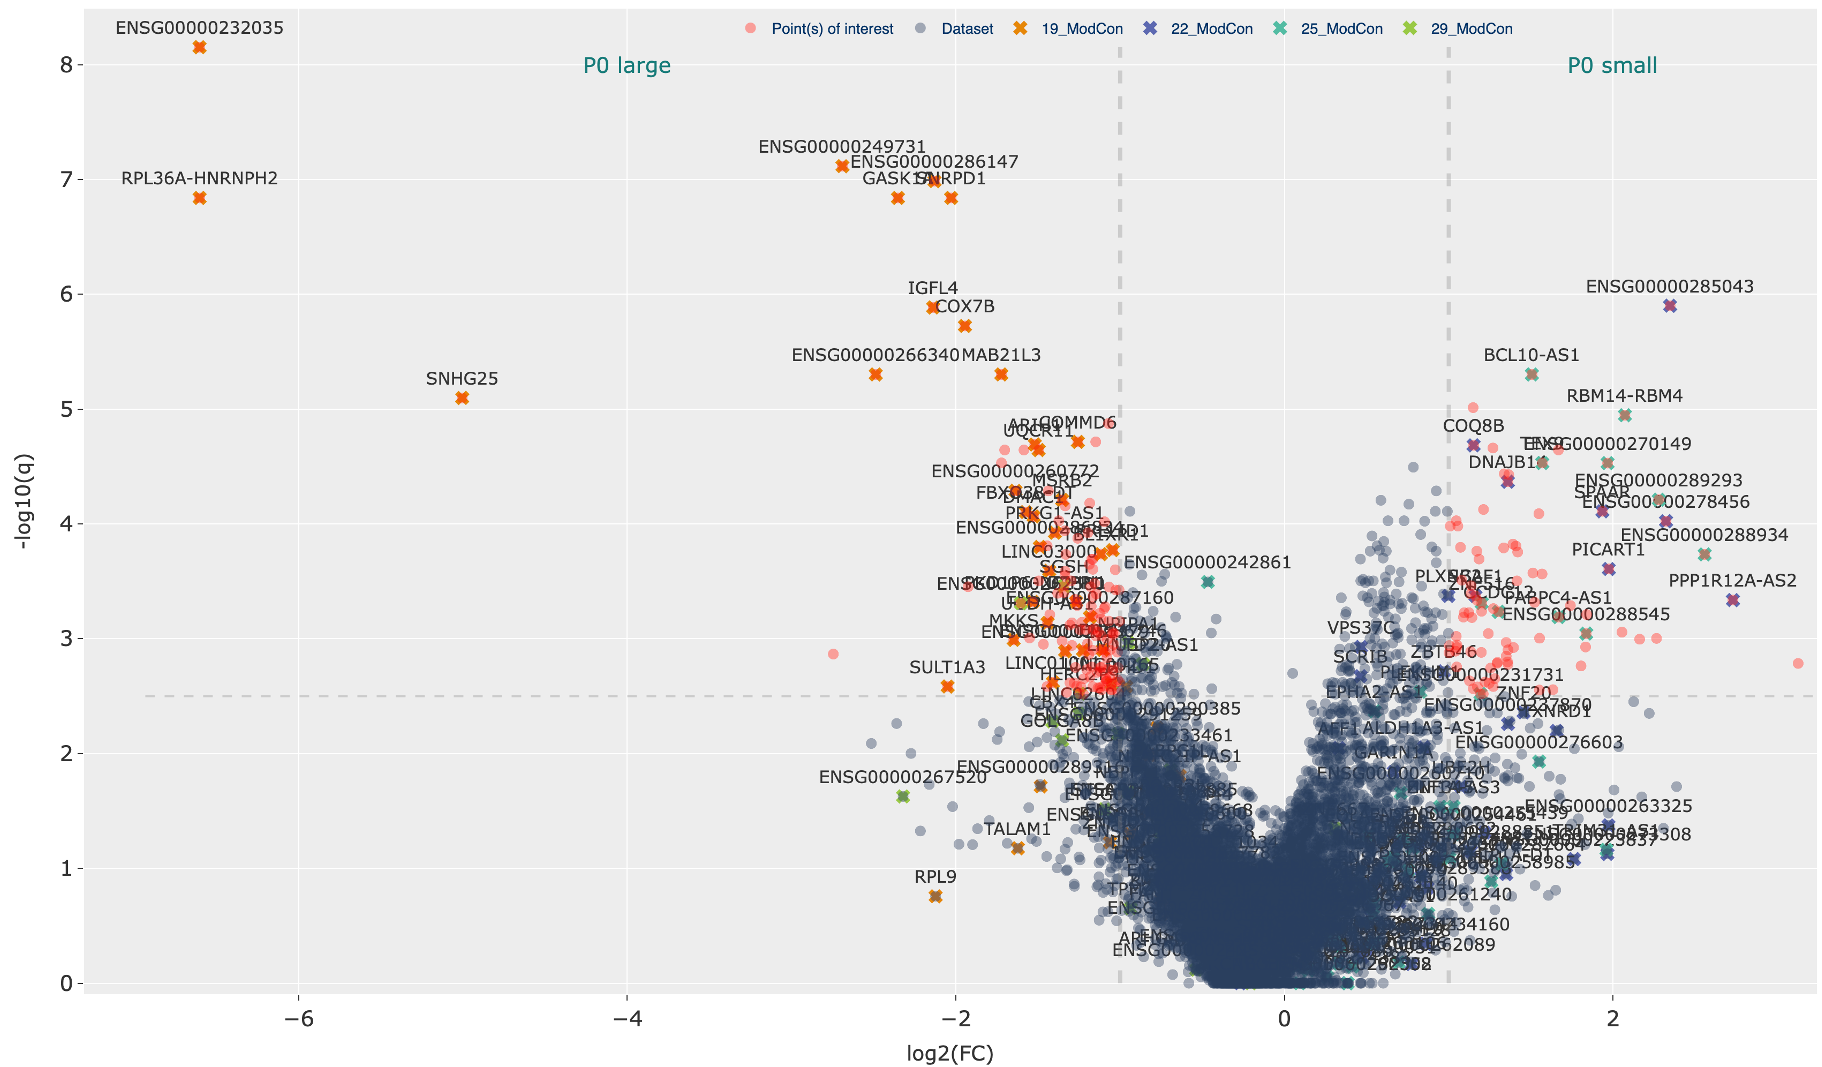
\includegraphics[width=1.0\textwidth,height=1.0\textheight,keepaspectratio]{Sections/Network_II/resources/non_tum/p0_split_dea.png}
    \caption[Volcano plot between the P0 splits]{Volcano plot showing the \acrlong{dea} for the comparison between the P0 split shown in the heatmap from \cref{fig:N_II:morph_non_tum}. The X-axis represents the difference in gene expression, $log_2(\text{fold\_change})$, while the Y-axis shows the significance of the change given by $-log_{10}(q)$. The genes on the right-hand side of the plot are those significantly expressed in the larger P0 group, while the points on the left-hand side are specific to the smaller P0 group. As in the previous Volcano plot there are several \acrshort{lncRNA} significantly expressed which highlight the novelty of the biological findings using the network approach.}
    \label{fig:N_II:p0_split}
\end{sidewaysfigure}

% Community characterisation
\subsection{Community characterisation} \label{s:N_II:comm_charact}

% Talking about the significance of the finding
In the two cases of the P0 and ABS-Ca splits, it can be observed which communities are driving the separation. It can also be noticed that the genes in these communities are found to be significantly expressed when performing the \acrlong{dea}. These two results have a two-fold implication. First, the network pipeline, and implicitly the hierarchical SBM, is able to find communities that are significantly expressed in some groups, demonstrating the power of the method. Secondly, the splits in the ABS-Ca and P0 samples indicate the opportunity to further explore new biological aspects of the differentiated status.

% Talk about the misfit communities
From the heatmap (\cref{fig:N_II:morph_non_tum}) and the two volcano plots (\cref{fig:N_II:diff_split,fig:N_II:p0_split}), it can be noticed that a few communities have a stronger influence on the splits. Communities 19 and 29 are specific to the small ABS-Ca and the large P0 groups, while community 25 is specific to the large ABS-Ca and small P0 groups. It can be seen in the clustering of the communities in \cref{fig:N_II:morph_non_tum} that these are clustered separately or with weaker communities (1 and 29, and 25 and 22).



% Linking the Volcano plots with the network.
Community 19 seems to be the leading driver of the splits, and to showcase the visualisation aspect of the networks, the genes forming the group are shown in \cref{fig:N_II:19_com}. The module comprises 123 genes, with the genes coloured in orange being the 50 with the highest ModCon scores\footnote{Note that there are 100 genes selected for the MEVs, but only 50 are highlighted in the community to ease visualisation.}, some of which were significantly expressed in the Volcano plots from earlier. In the case of the ABS-Ca split, genes like \textit{TALAM1}, \textit{SNRPD1}, \textit{COX7B}, or even \textit{ENSG0000023205} are in the top 50 ModCon. For the P0 split, nodes like \textit{SNHG25}, \textit{IGFL4}, \textit{MAB21L3}\footnote{Gene \textit{MAB21L3} is trimmed to \textit{MAMB21L.} in the network as part of the automatic process to shorten the longer gene names and help with visualisation}, and again \textit{ENSG0000023205}. The connection between ModCon and the genes found through the DEA affirms the utility of using the network and its usefulness to analyse subsets of genes. Similar analysis was performed for communities 25 and 29, which can be found in \cref{ap:N_II:coms} from the Appendix.



% Community characterisation
Apart from the differences in the P0 and ABS-Ca samples, the heatmap shows that the communities can be labelled as tissue-specific. For example, communities 0, 2, 3, 4, 5, 7, and 6 are all more enriched in the P0 samples, while communities 11, 12, 34, 10, 14, 9, 13, 21 are enriched in the UD samples. Towards the bottom of the heatmap, communities 20, 26, 28, 31, 27, 24, 30, and 32 are enriched in differentiated tissue. Communities 19 and 29, which drive the ABS-Ca/P0 split, do not belong to any group and are classified as 'Misfit,' while community 18 is enriched in both UD and P0 samples.


\begin{figure}[H]    
    \centering
    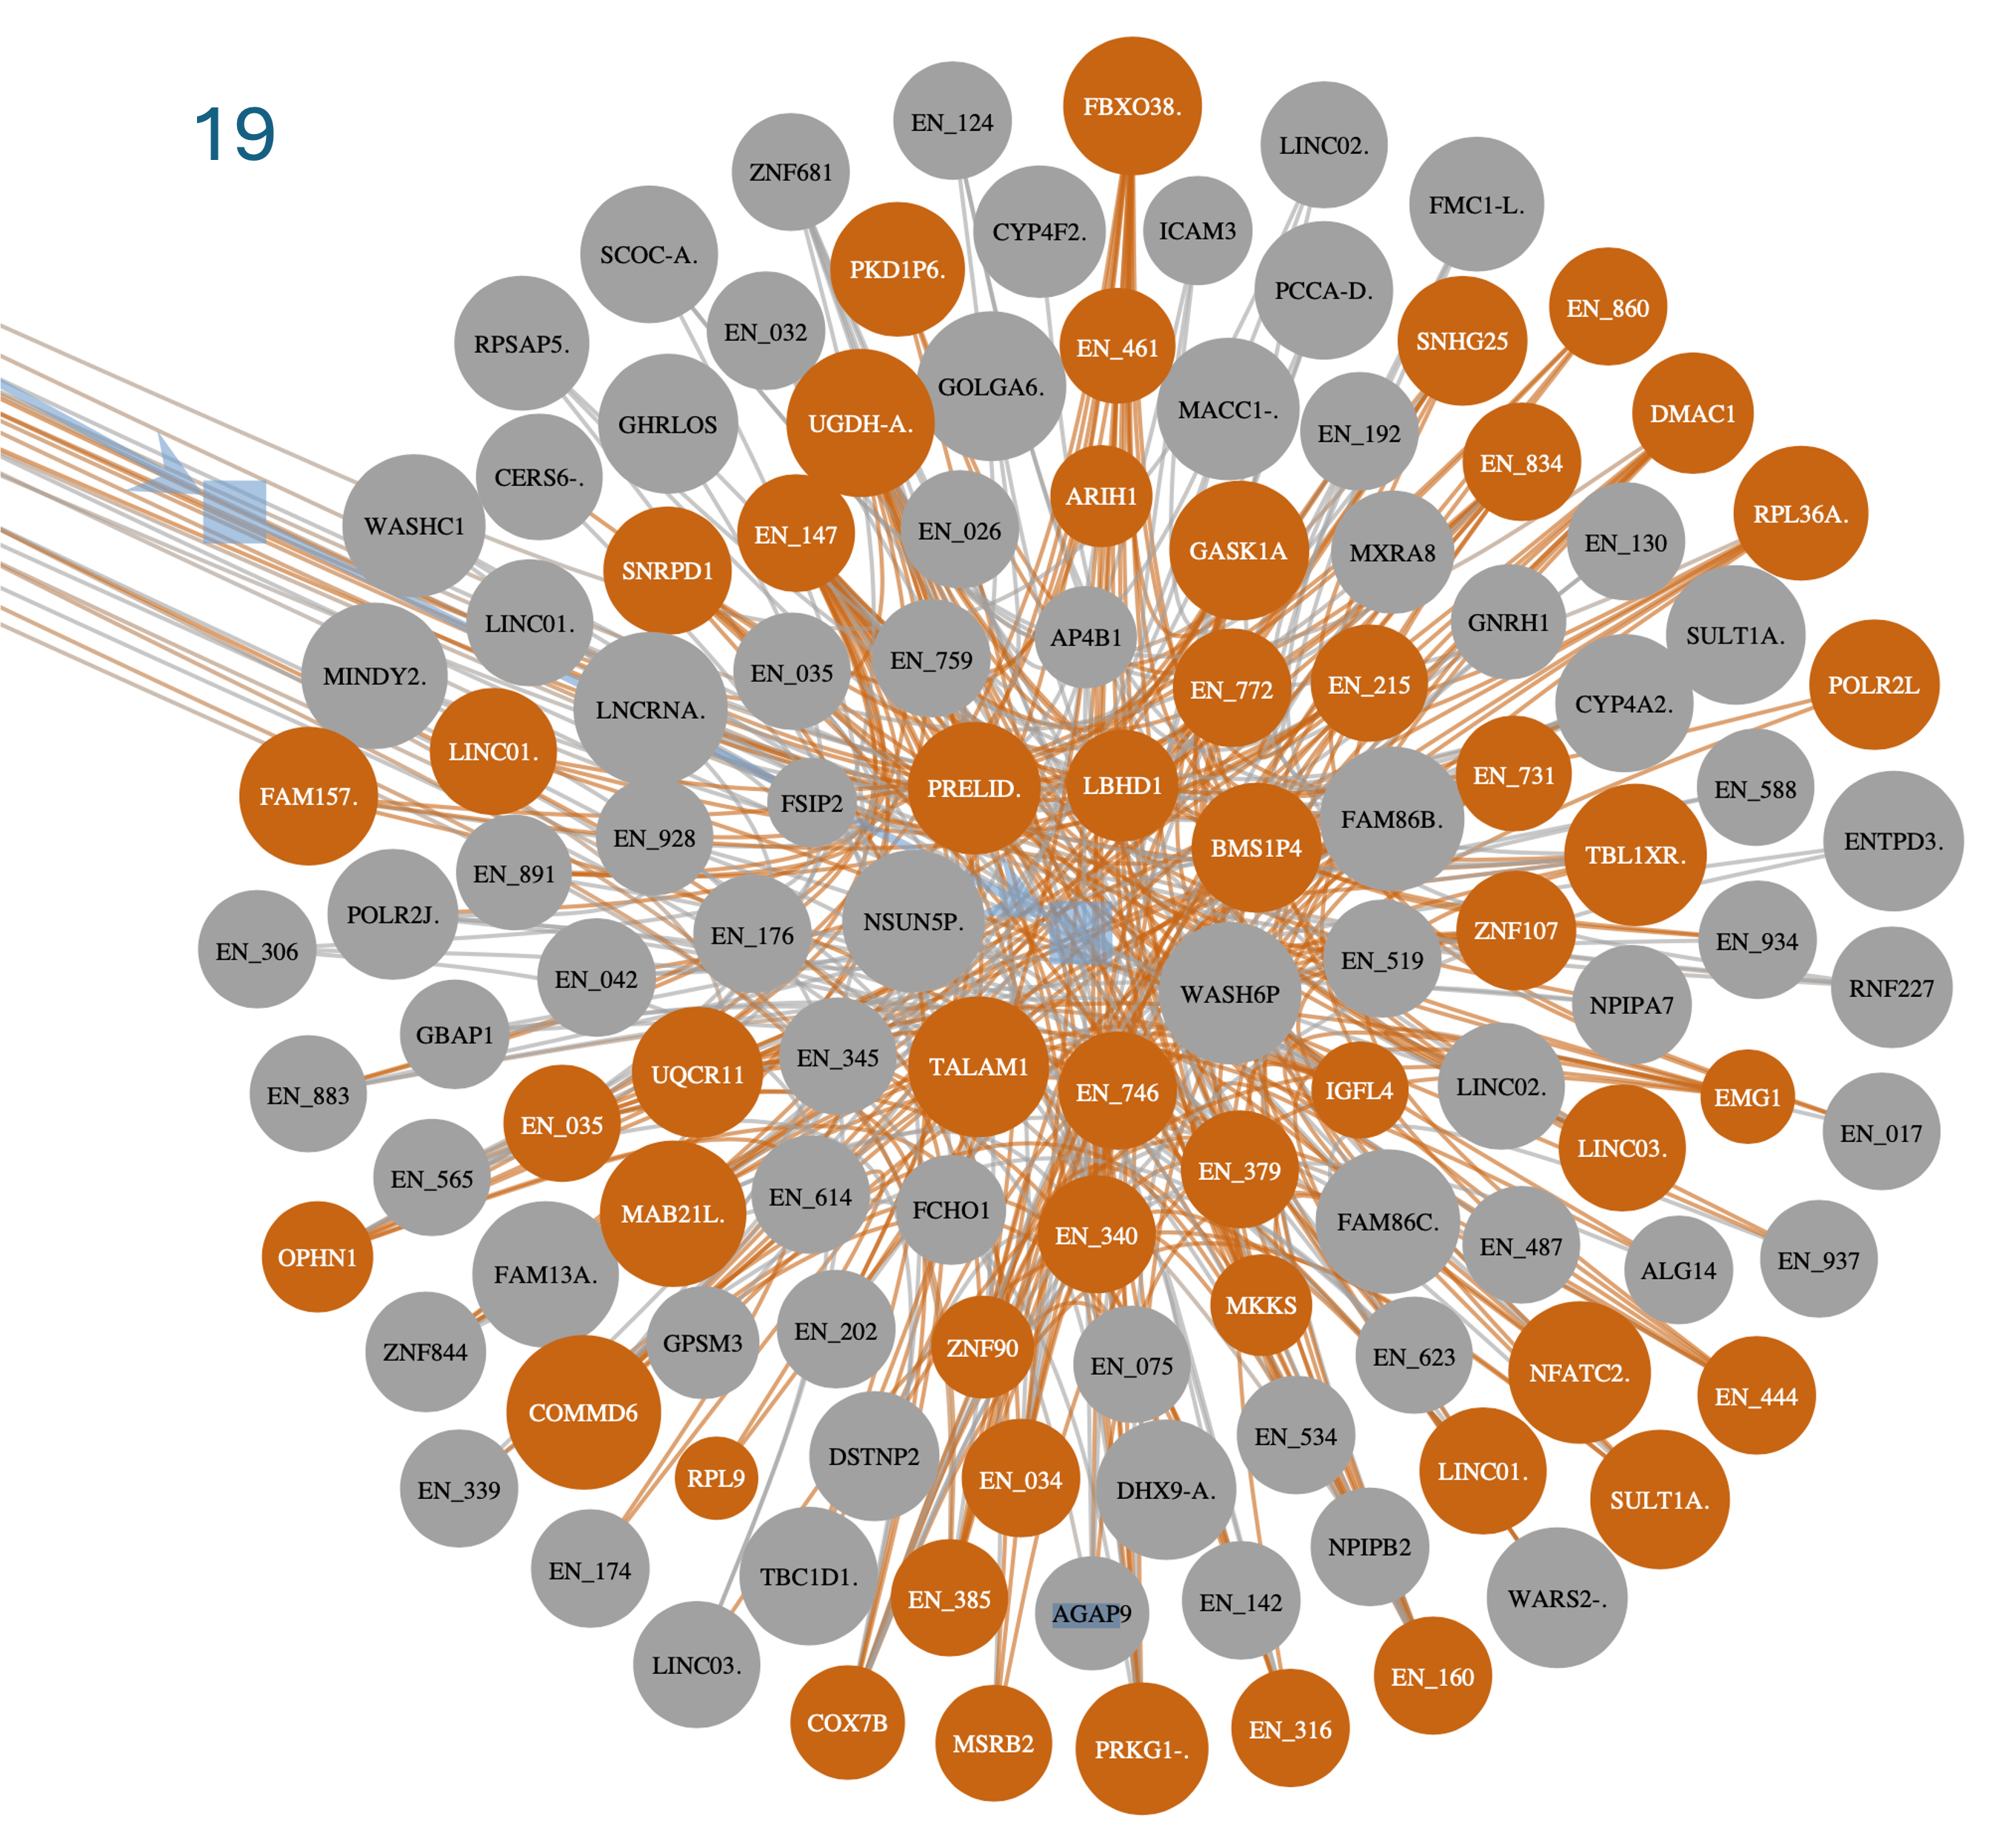
\includegraphics[width=1.0\textwidth,height=1.0\textheight,keepaspectratio]{Sections/Network_II/resources/non_tum/19_com.png}
    \caption[Community 19]{Community 19 (along with 29 and 25) drives the splits in the tissue differentiation datasets. This community is enriched in the small ABS-Ca and the large P0 subgroups from \cref{fig:N_II:non_tum_sankey_comp}. The standard network is generated from 5000 genes, with no weight modifier, and the \acrshort{hsbm} was applied. The community contains 123 genes, of which the 50 with the highest ModCon scores are highlighted in orange. To aid visualisation, some of the gene names were trimmed: for those with longer names, the first 5 letters were kept, while for 'ENSG...' like nodes, "EN\_" and the last 3 digits were retained. The community contains many Ensembl genes or \acrshort{lncRNA} highlighting an additional layer of complexity to bladder biology. See the network representation of community 25 (\cref{fig:ap:com_25}) and 29 (\cref{fig:ap:com_29}).}
    \label{fig:N_II:19_com}
\end{figure}


% Why I am putting this here
Assigning them a tissue function may help in further analysis of the MIBC subtypes. To further validate them, DEA was performed between the three datasets: ABS-Ca, UD, and P0. For each community, the genes selected by ModCon (top 100) were plotted against the volcano plots, as in \cref{fig:N_II:p0_split,s:N_II:diff_split}. This allows for confirmation of the 'trends' in the communities. The results can be seen in the cluster tree in \cref{fig:N_II:cluster_tree}, generated using \textit{clustree} package \citep{Zappia2018-bt}.

% Summary of the work
The cluster tree represents a summary of the work done in this section, where each community was labelled by their enrichment in the tissue-differentiated samples. The communities found at the lowest level (0) are also detectable with the standard SBM; the hierarchical version simply performs an additional clustering from bottom to top. This means that the communities from level 0 SBM are applied, resulting in the 14 communities at level 1, and this continues until there is one single community found, in this case, until level 4. All the analysis performed in this section is at level 0, and then the information is propagated upwards.

% Commenting on the cluster tree
It can be observed that at level three, there are different communities almost corresponding with the differentiated properties of the datasets used. It is not surprising to see that P0 and ABS-Ca (Diff) are grouped together as they are 'closer' on a differentiation spectrum. One can also notice that there is a difference in the grouping performed by the traditional hierarchical clustering in the heatmap from \cref{fig:N_II:morph_non_tum} and the SBM version in the cluster tree \cref{fig:N_II:cluster_tree}. This is because the hSBM uses all genes, while the standard hierarchical clustering receives the MEVs for a selected few via ModCon.


% Talk about the misfits and comment the clustertree

\begin{figure}[H]    
    \centering
    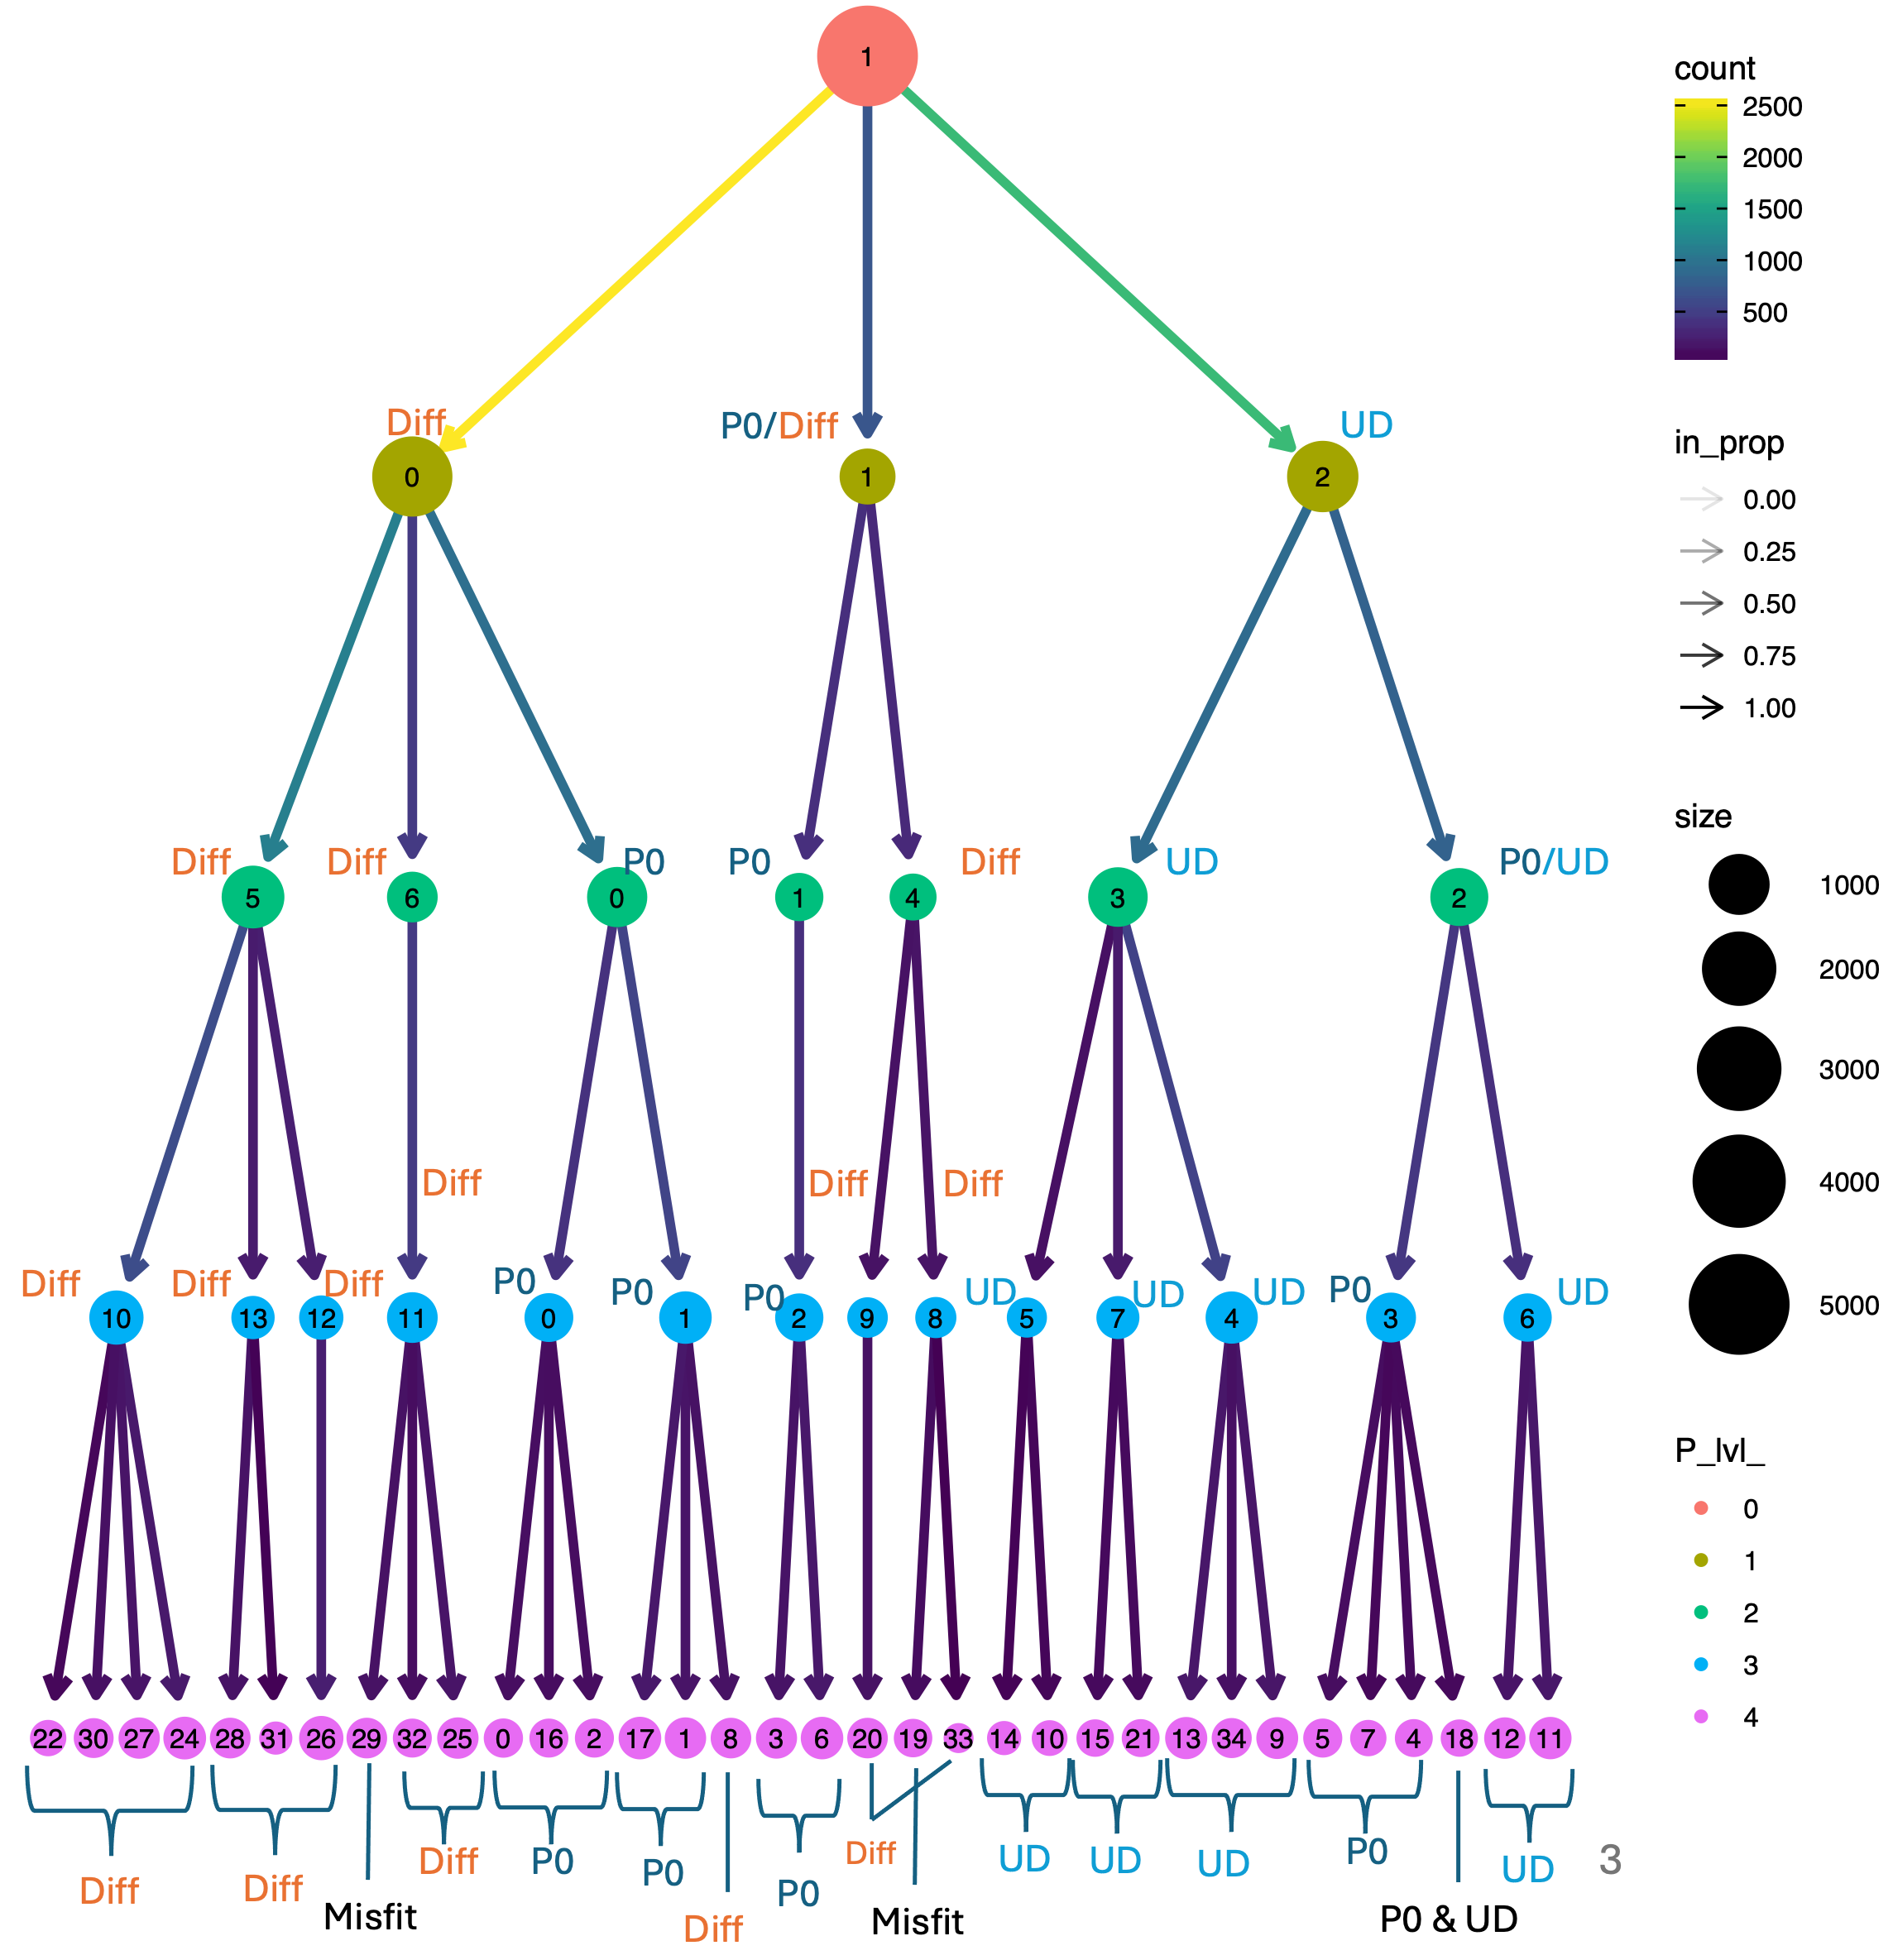
\includegraphics[width=1.0\textwidth,keepaspectratio]{Sections/Network_II/resources/non_tum/clustertree_labels.png}
    \caption[Cluster tree: non-tumour and bladder differentiation]{Cluster tree representation of the communities found through \acrshort{hsbm} \citep{Peixoto2014-yb}. There are 5 levels, and the size of the dots represents the size of the communities. The communities at the bottom layer were classified as Diff (ABS-Ca), UD, P0, or Misfit via \acrfull{dea}, covered in \cref{s:N_II:comm_charact}. The labels for the upper levels were propagated from the bottom. This is a summary of the community analysis in \cref{s:N_II:comm_charact} with their enrichment in the three non-tumour datasets.}
    \label{fig:N_II:cluster_tree}
\end{figure}



% 
\subsection{MIBC split} \label{s:N_II:tum_split}

% Introduce the work
The non-tumour stratification yields new groups in two of the three datasets used to built the graph but how capable is the standard network to subtype the MIBC cohort from TCGA? This part of the chapter attempts to answer the question by using the same network presented earlier: 5000 most varied genes, 3 edges per standard gene and 6 per TF and using hierarchical SBM. The main difference is that the stratification is performed on the tumour samples rather then the non-tumour dataset. This means a different dataset is used from which the network was built and the integrative MEV (iMEV) is used, see \cref{s:N_II:iMEV}.

% Describe the figure
The resultant MEVs are analysed with Morpheus \citep{Broad-Institute2016-tn}, \cref{fig:N_II:tum_morph}, which are first quantile normalised, then the hierarchical clustering with average linkage and cosine distance is applied. Dendrogram cuts of 10 for samples and 6 communities are used as higher values lead to smaller communities (mostly of 1-2 samples). At the top is shown the classifications by the work on cluster analysis from \cref{s:cs:bio_interp}, TCGA, consensus and Lund \citep{Robertson2017-mg,Kamoun2020-tj,Marzouka2018-ge}. On the right hand side the "Diff Type" represents the community labelling from the last section.

% Talk about the splits
The heatmap in \cref{fig:N_II:tum_morph} demonstrates that MIBC is categorised into the two canonical groups: Luminal on the left (green by Consensus/TCGA) and Basal (mostly blue by Consensus/TCGA) on the right. The Luminal group is further divided into six subgroups, two of which consist of a few samples (n=3 for both), and three larger groups (n=92, n=74 and n=13). The remaining four clusters are Basal subgroups, with one group being particularly enriched in Stroma according to TCGA. Notably, there is no evidence of the three Basal splits by the \acrfull{ifn} response observed in the first part of the project, nor a distinct separation of a Mes-like group as discussed in \cref{s:N_I:sel_pruning}. This might be explained by that the non-tumour dataset does not include samples with a strong immune response. Observing the top dendrogram, it is evident that as the cut increases, more groups emerge. A notable mention is the NE group on the left side of the Basal group. However, artificially increasing the dendrogram cut does not enhance the outcome.

% Talk about the communities
Shifting the focus on the communities, the previous highlighted 19, 25 and 29 have a less clearer impact on the tumour stratification. These groups may be involved in the split of the luminal group \cref{fig:N_II:tum_morph}, but there are clearer communities that make the separation. For example, community 9, 13, 15, 21 classified as UD, are more enriched\footnote{This refers to the genes that are present in the mentioned communities are more expressed in one group than the other} in the Basal than the Luminal groups while 8 (diff), 16 (p0), 17 (p0) are specific to the Luminal group and not to the Basal. Communities 1, 29, 25, 27 (diff) seems to be specific the Luminal group on the left-hand side with a low expression in all the Basal group. 

% Conclusion
The heatmap in \cref{fig:N_II:tum_morph} indicates that most of the diff and P0 communities are specific to the Luminal groups which are known to be closer to the healthy bladder differentiated tissue. While the UD modules are enriched in the Basal subtype which have an undifferentiated, squamous phenotype. Having the ability to trace group of genes to the MIBC splits shows the power of the network approach and validates one of the initial hypothesis where communities can be used to explain the biology of the subgroups.

% Dealing with exception
There are a few exceptions, such as communities 4, 5, 10, and 12, which are generally enriched across all samples, with only a few scattered exceptions in the luminal subgroups (dendrogram\_cut 4, 5, 6, 7). Community 7, which was associated with P0, appears to be unexpectedly enriched in the Stroma subgroup on the right-hand side. This is surprising, as the non-tumour samples were separated from the stroma cells, suggesting the possibility of shared gene expression between stroma-classified and P0 samples. These exceptions may be explained by the gene expression differences between the non-tumour samples and TCGA's MIBC cohort.

The analysis illustrates the potential of the network approach and using communities found in a non-tumour network and then used to stratify the MIBC. While these are not powerful enough to further stratify the MIBC in new groups, it shows that the communities can be used to focus the analysis on groups of genes. For example, one possible next step is to further investigate what are the genes in communities 4, 5, 10 and 12 as well as what makes the most left luminal community to be separated. However, due to the limited time in the PhD the efforts were concentrated on improving the reward modifier which is explored in the next section.

\begin{sidewaysfigure}[ht]
    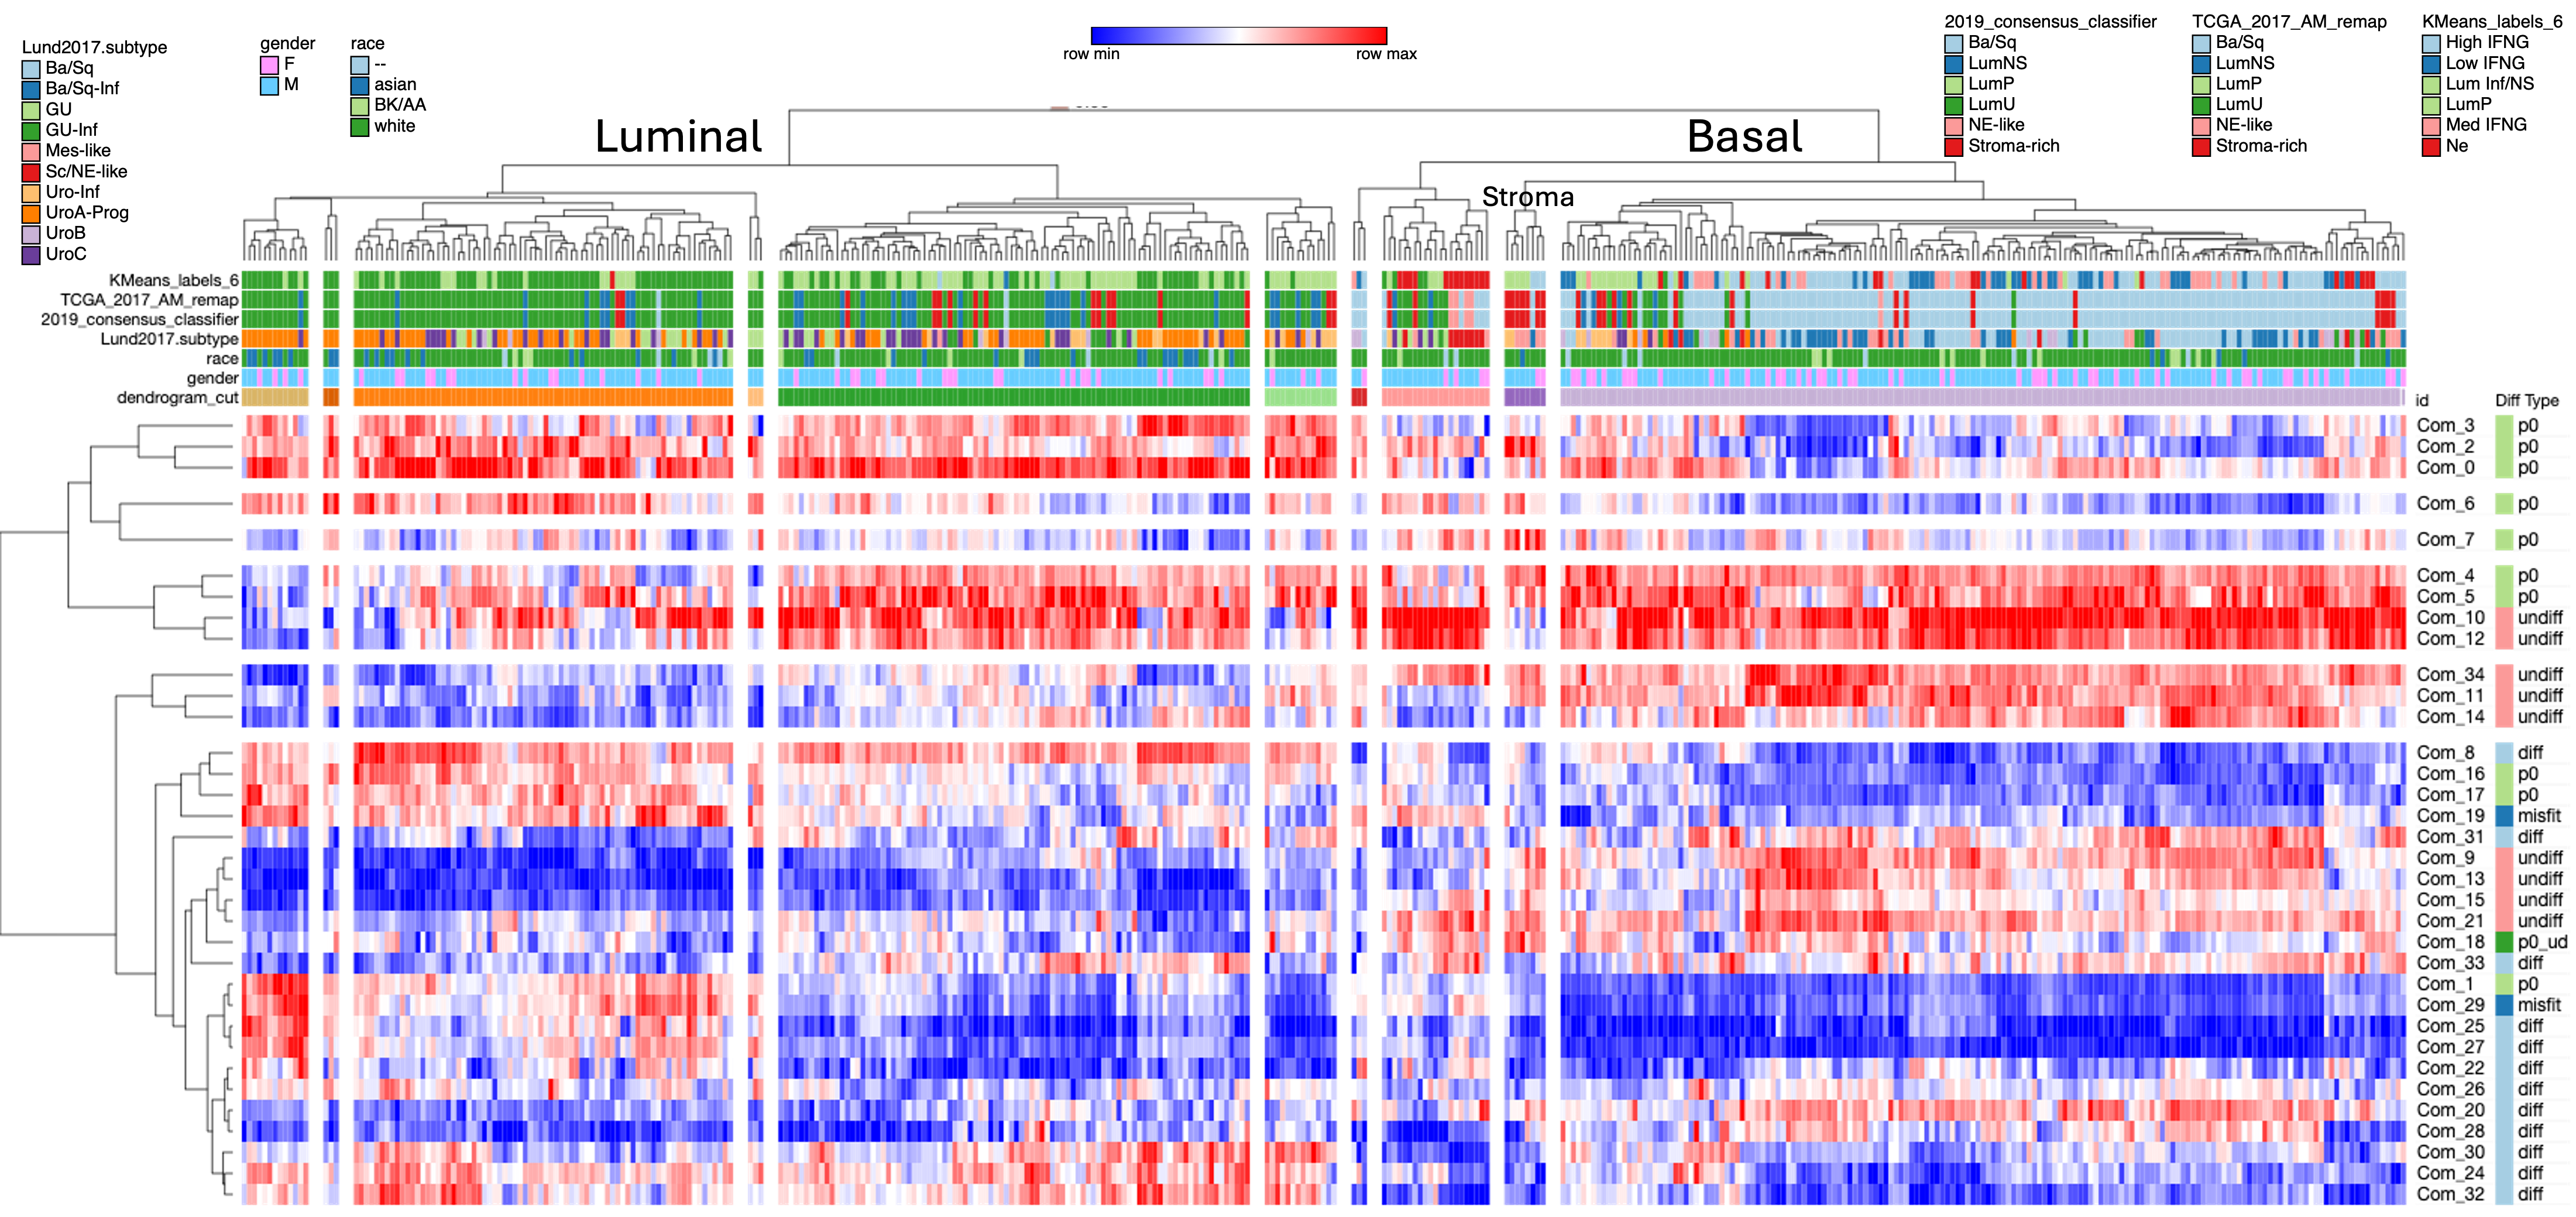
\includegraphics[width=1.0\textwidth,keepaspectratio]{Sections/Network_II/resources/non_tum/iMev_3_3_cs_13_horiz.png}
    
    \caption[Heatmap: MIBC subgroups derived from non-tumour network]{Heatmap showing both the MIBC subtypes and the grouped communities by applying the hierarchical clustering with average linkage and cosine distance on the MEVs. There are four metadata shown at the top: gender (Female/Male), race (asian, black/afro-american and white), and the three referential classifier used in the project: Lund, consensus, TCGA \citep{Marzouka2018-ge,Kamoun2020-tj,Robertson2017-mg} as well as the work form the first chapter \cref{s:cs:bio_interp}. A dendrogram cut of 10 for samples and 6 for communities was used as higher values lead to more smaller communities. On the right hand side the "Diff Type" represents the community labelling from \cref{s:N_II:comm_charact}.
    }
    \label{fig:N_II:tum_morph}
\end{sidewaysfigure}


\subsection{Summary}


% Introduction and discussion of the findings in the non-tumour dataset
This section has a dual purpose: to validate the new network pipeline and to test if the communities can be traced to the MIBC subgroups derived. The methods introduced cannot only split the dataset by the three differentiation statuses, further validating the pipeline, but are also capable of identifying new divisions in the P0 and ABS/Ca datasets, demonstrating the power to uncover new relevant biology. There is a strong link between the graph communities and the results from \acrlong{dea}, which further explored the tissue differentiation splits (see \cref{fig:N_II:p0_split,fig:N_II:diff_split}), where genes extracted from communities were significantly expressed. The transparency of the method is crucial to advancing the understanding of the molecular biology of the bladder.


% Refer to the ENSG splits
Remarkably, the network approach can isolate distinct groups within the ABS-Ca dataset, such as a paediatric group and a male-dominant group. It is also important to highlight that most of the genes responsible for the splits in the P0/ABS-Ca datasets were identified by their Ensembl IDs, indicating the unexplored aspects of bladder biology. The large number of poorly characterised genes may be due to the non-tumour dataset, which has been less researched than tumour datasets. The presence of many significantly expressed Ensembl genes underscores the potential for uncovering new biological insights and demonstrates that using a non-tumour representation adds another level of unexplored biological territory.

% MIBC result
This results section presents the first attempt to use the network representation of the non-tumour dataset to stratify \acrlong{mibc}. The two main groups, Basal and Luminal, were identified using the network approach and some smaller groups, such as the Stroma-rich group. The MIBC stratification reveals different subtypes with more subgroups in the Luminal group compared to the subgroups found in the previous chapter (\cref{s:clustering_analysis}), which identified a three-way Basal split based on \acrlong{ifn}.

The network approach enables tracing the communities responsible for subtyping the ABS-Ca and P0 datasets and the MIBC. This is a remarkable and powerful feature of the method developed in this project, as it eases interpreting and understanding the newly discovered groups. It also encourages further development of such techniques to enable additional data integration, as discussed in the next section.

% Summary
Overall, this results chapter represents a concentrated effort on the non-tumour dataset, validating and showcasing the advantages of the new network pipeline. In doing so, two new splits in the ABS-Ca and P0 datasets have been identified, which may help reveal new biology. It also demonstrates that the network approach has the potential to identify new MIBC groups and trace them back to the communities responsible for the division. The next chapter will focus on integrating mutation data and the stratification of MIBC.



% It is also important to highlight that most of the genes responsible for the splits in the P0/ABS-Ca datasets were Ensemble named genes, showing the uncharted side of bladder biology. It is remarkable that this method is capable of isolating a paediatric group of patients and a male-dominant group in the ABS-Ca dataset, and that the genes selected with ModCon are present in the differential expression analysis. The large number of Ensemble genes in the DEA signals that the genes

% The large number of Ensemble name genes is due to the use of the non-tumour dataset, which has been less researched compared to the genes involved in tumour datasets. 
